%7
\section{Paketdetails}
\begin{figure}[H]
\centering
\includegraphics[width=1\textwidth]{img/7-paketdetails}
\caption{Klassendiagramm zur detaillierten Beschreibung der strukturellen Gliederung}
\label{Paketdetails}
\end{figure}

%7.1 Paket Robot
\subsection{Paket \textit{Robot}}
	Im Folgenden beschreiben wir die wichtigen Klassen des Pakets \textit{Robot} 
	und ihre zugehörigen wichtigen Methoden, sowie ihre Interaktion untereinander. 


	%7.1.1 RobotController
	\subsubsection{Beschreibung der Klasse \textit{RobotController}}
%		\begin{figure}[H]
%		\centering
%		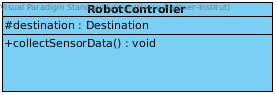
\includegraphics[width=0.6\textwidth]{../images/Iteration0_Entwurf_7-1-1_Klasse_RobotController}
%		\caption{\textcolor{blue}{Durch eigene Diagramme ersetzen}}
%		\label{BeschreibungKlasse1}
%		\end{figure}
		
		%#destination : Destination
		Die Klasse \textit{RobotController} ist die Hauptklasse des \textit{Robots}, 
		da sie den aktuellen Zustand des \textit{Robots} enthält.
		So hat diese Klasse die Möglichkeit, maximal einen \textit{Task} zu speichern. 
		Dieser \textit{Task} kann ein vom \textit{Server} zugeteiltes Ziel sein, 
		der dem \textit{Robot} zugehörige \textit{Charger}, oder gerade kein Ziel, 
		also \texttt{null} sein. Nur wenn der \textit{Robot} gerade keinen \textit{Task} 
		gespeichert hat, kann er neue Aufträge vom \textit{Server} annehmen.

			%7.1.1.1 #collectSensorData():void
			\paragraph{Beschreibung der Methode \texttt{getSensorData}}
			Der Server kann einen \textit{Robot} dazu auffordern, ihm seine Soensordaten zu schicken. Der \textit{Robot} fragt dann seine Hardwareschnittstelle mittels der Methode \texttt{readSensors} 
			nach seiner Position und seinem Akkustand an und gibt diese Informationen zusammen mit einer Information über seinen aktuellen Zustand (also seinem aktuellen \textit{Task}) zurück an den \textit{Server}. Dazu wird natürlich zunächst eine \textit{Message} verfasst, welche dann über die im \texttt{Common}-Paket enthaltene Schnittstelle über den \textit{IWlanAdapter} mit der Methode \texttt{send} verschickt wird.
			
			\paragraph{Beschreibung der Methode \texttt{informAboutArrival}}
			Diese Methode wird immer dann aufgerufen, wenn der \textit{Robot} die nächste \textit{Position} von seinem aktuellen \textit{Task} erreicht hat. Übergeben wird dabei genau diese \textit{Position}. Der \textit{Robot} verfasst eine neue \textit{Message} und schickt sie über die \textit{IWlanAdapter}-Schnittstelle an den \textit{Server}. 
			
	%7.1.2 DrivingSystem
	\subsubsection{Beschreibung der Klasse \textit{DrivingSystem}}
%		\begin{figure}[H]
%		\centering
%		\includegraphics[width=0.6\textwidth]{../images/Iteration0_Entwurf_7-1-2_Klasse_DrivingSystem}
%		\caption{\textcolor{blue}{Durch eigene Diagramme ersetzen}}
%		\label{BeschreibungKlasse1}
%		\end{figure}
		
		%#currentSpeed:float
		Diese Klasse beschreibt den aktuellen Zustand des Fahrsystems des \textit{Robots}. 
		Es sind Informationen über die aktuelle Geschwindigkeit enthalten und die Methode, 
		die gerade ausgeführt wird, gibt Auskunft über die aktuelle Beschäftigung des \textit{Robots}.

			%7.1.2.1 	#driveToDestination(destination: Destination, arrivalHandler: ArrivalHandler): void
			\paragraph{Beschreibung der Methode \texttt{driveToDestination}}
			\begin{figure}[H]
			\centering
			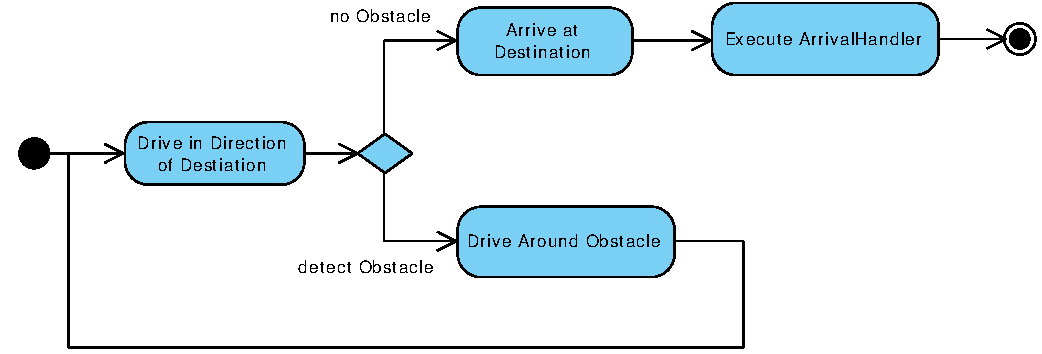
\includegraphics[width=1\textwidth]{img/1-Entwurf-7-1-methode_driveAroundObstacle}
			\caption{Aktivitätsdiagramm zur Methode \texttt{driveToDestination}}
			\label{AktivitaetDriveToDestination}
			\end{figure}

			Wenn diese Methode aufgerufen wird, macht der \textit{Robot} sich auf den Weg zur 
			übergebenen \textit{Destination}. Wenn der \textit{Robot} an dieser \textit{Destination} 
			angekommen ist, wird die \texttt{arrive}-Methode des übergebenen \textit{ArrivalHandlers} ausgeführt. 
			Wenn sich ein \textit{Obstacle} auf dem Weg befindet, wird die Methode \texttt{driveAroundObstacle} 
			aufgerufen, bis das \textit{Obstacle} umfahren wurde.
			
			Abbildung \ref{AktivitaetDriveToDestination} zeigt ein entsprechendes Aktivitätsdiagramm.

			%7.1.2.2    -driveAroundObstacle(destination: Destination): void
			\paragraph{Beschreibung der Methode \texttt{driveAroundObstacle}}
			\begin{figure}[H]
			\centering
			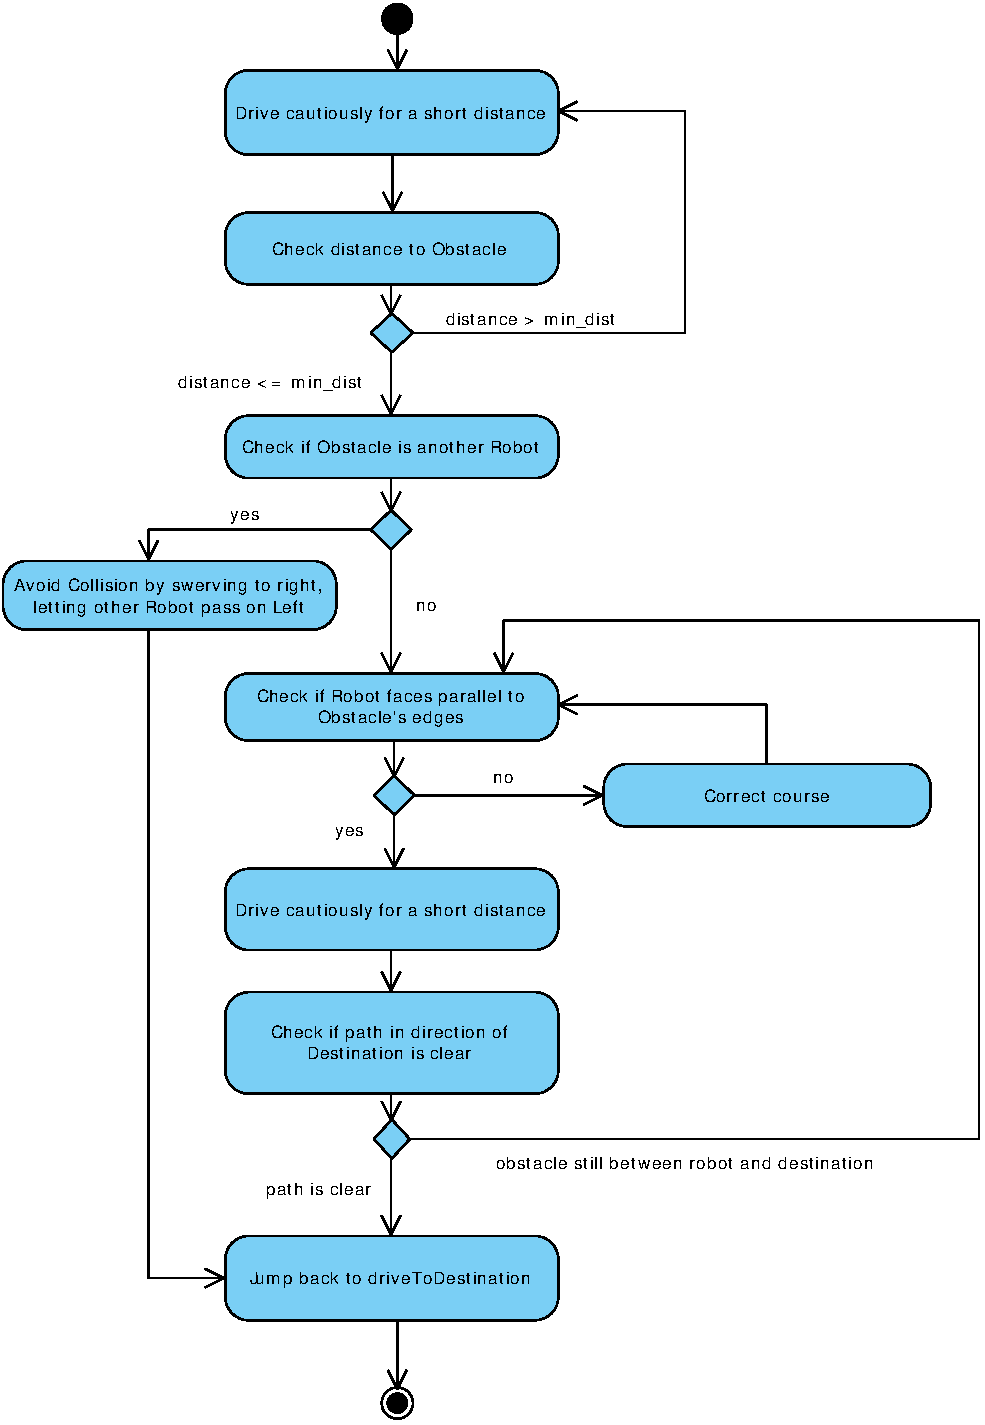
\includegraphics[width=0.95\textwidth]{img/1-Entwurf-7-driveAroundObstacle}
			\caption{Sequenzdiagramm zur Beschreibung der Methode \texttt{driveAroundObstacle}}
			\label{SequenzDriveAroundObstacle}
			\end{figure}

			Diese Methode wird von \texttt{driveToDestination} mit des Position eines \textit{Obstacles} aufgerufen, 
			wenn ein \textit{Obstacle} zu umfahren ist. 
			Im Spezialfall, dass es sich bei dem \textit{Obstacle} um einen anderen \textit{Robot} handelt, merken dies beide wenn sie sich nähern und weichen beide nach rechts aus. Im Allgemeinen entscheidet sich der \emph{Robot} zunächst, ob er links oder rechts an dem \textit{Obstacle} vorbeifährt, 
			und hält sich dann mithilfe seiner Sensoren immer auf einem bestimmten Abstand zum Hindernis, bis zwischen 
			\textit{Obstacle} und der Luftlinie zur \textit{Destination} genug Platz für den \textit{Robot} ist.
			
			Abbildung \ref{SequenzDriveAroundObstacle} zeigt ein entsprechendes Sequenzdiagramm. Dabei ist \texttt{min\_dist} eine vorher festgelegte Konstante, welche die Mindestdistanz, die der \textit{Robot} halten muss, wenn er an einem \textit{Obstacle} vorbeifährt, speichert.
	
\pagebreak
	
%7.2 Paket Server
\subsection{Paket \textit{Server}}
%\begin{figure}[H]
%	\centering
%	\includegraphics[width=0.6\textwidth]{../images/Paketdetails.png}
%	\caption{\textcolor{blue}{HIER KOMMT DAS Server - PAKETDIAGRMAM HIN}}
%	\label{Paketdetails}
%	\end{figure}
	Im Folgenden werden die wichtigen Klassen des Pakets \textit{Server} 
	und ihre zugehörigen Methoden sowie ihre Interaktion untereinander beschrieben. 


	%7.2.1 TaskSystem
	\subsubsection{Beschreibung der Klasse \textit{TaskSystem}}
		%	-taskDistribution
		Das \emph{TaskSystem} des \emph{Servers} verarbeitet alle \emph{Tasks}, die es mit der Zuordnung vom \emph{RobotControlSystem} übergeben bekommt. Dafür besitzt es eine Struktur, die die \emph{taskDistribution} intern verwaltet und somit die \emph{Tasks} und die jeweils zugeordneten \emph{Robots} kennt.
		
		%7.2.2.1	~assignTask(virtualRobot : VirtualRobot, destination : Destination): void
			\paragraph{Beschreibung der Methode \texttt{assignTask}}
			Die Methode \texttt{assignTask} führt die Zuordnung und Abspeicherung der \emph{Robots} und \emph{Tasks} bzw. \emph{Destinations} durch. Sie wird aufgerufen, wenn \texttt{chooseRobot} einen passenden \textit{Robot} gefunden hat, der einen \textit{Task} entgegennehmen kann. Die Methode \texttt{assignTask} schickt dann eine neue \textit{Message} über den \textit{IWlanAdapter} an den \textit{Robot}, welche den \textit{Task} enthält.
			
	%7.2.2 RobotControlSystem
	\subsubsection{Beschreibung der Klasse \textit{RobotControlSystem}}
		Das \emph{RobotControlSystem} sorgt bei eingehenden \emph{Tasks} dafür, dass ein passender \emph{Robot} ausgewählt wird. Diese Information übergibt es dann an das \emph{TaskSystem}, das für die endgültige Zuordnung zuständig ist.
	
			%7.2.1.1	~chooseRobot(destination: Destination): void
			\paragraph{Beschreibung der Methode \texttt{chooseRobot}}
			Die Methode \texttt{chooseRobot} wählt für den aktuell eingegangenen \emph{Task} einen \emph{Robot} aus. Dazu fragt es die Sensorwerte der verschiedenen \emph{Robots} ab und wählt den am besten geeigneten aus.
			
			\paragraph{Beschreibung der Methode \texttt{denyHospitalRequest}}
			Laut Aufgabenstellung kann das Krankentransportsystem nur neue Aufträge vom \textit{Hospital} entgegennehmen, wenn auch mindestens ein \textit{Robot} den \textit{Patient} erreichen könnte. Falls der \textit{Server} über die Schnittstelle \textit{IHospitalInputHandler} also einen \textit{Patient} holen soll, der für das System unerreichbar ist, muss das System dies dem \textit{Hospital} mitteilen, damit dieses weiß, dass es nach einer alternativen Lösung suchen muss.
			
			
			\paragraph{Beschreibung der Methode \texttt{acceptHospitalRequest}}
			Diese Methode wird immer dann aufgerufen, wenn der \textit{Server} eine neue Anfrage vom \textit{Hospital} über die \textit{IHospitalInputHandler} bekommt, und anschließend im Rahmen von \texttt{chooseRobot} klar wird, dass es einen geeigneten \textit{Robot} gibt, der den \textit{Patient} auch erreichen kann. Es wird eine neue \textit{Message} verfasst und über die \textit{IWlanAdapter}-Schnittstelle verschickt, die dem \textit{Hospital} mitteilt, dass ein \textit{Robot} zum \textit{Patient} geschickt wurde, und dieser demnächst eintreffen wird.
